\begin{enumerate}[(a)]
\item It's extremely important to first understand the way the data are recorded. Let's have a look at few lines of the data

\begin{spacing}{1.2}
\begin{footnotesize}
\begin{verbatim}
> ########################################
> ### LAB 9: Time-dependent covariates ###
> ########################################
> 
> # (a)-(i): Read the famous Stanford heart transplant data set in R
> stanford = read.csv("C:/Applied_Survival_Analysis_Jan2016/lab9/data/stanford.csv")
> head(stanford)
  patid year age fail time surgery transplant waitime
1     1   67  30    1   50       0          0      NA
2     2   68  51    1    6       0          0      NA
3     3   68  54    1   16       0          1       1
4     4   68  40    1   39       0          1      36
5     5   68  20    1   18       0          0      NA
6     6   68  54    1    3       0          0      NA
\end{verbatim}
\end{footnotesize}
\end{spacing}
Patient 1 never received a new hearth. He/she died 50 days after the acceptance while still being on the waiting list. 
Please, make sure you know how missing values are coded in \verb|R|. In \verb|R|, 
\verb|NA| does not denote a string (character) but rather denotes a missing value. Be careful with this. 
\begin{enumerate}[(i)]
\item We now perform a naive analysis of the effect of transplantation on the hazard of death by considering the transplantation status as fixed binary covariate. Such a model is straightforward to fit using the methods we've known so far. 
\begin{spacing}{1.2}
\begin{footnotesize}
\begin{verbatim}
> # Fit a naive Cox model
> library(survival)
> naiveCox = coxph(Surv(time,fail) ~ transplant,data = stanford)
> summary(naiveCox)
Call:
coxph(formula = Surv(time, fail) ~ transplant, data = stanford)

  n= 103, number of events= 75 

              coef exp(coef) se(coef)     z Pr(>|z|)    
transplant -1.3238    0.2661   0.2438 -5.43 5.63e-08 ***
---
Signif. codes:  0 ‘***’ 0.001 ‘**’ 0.01 ‘*’ 0.05 ‘.’ 0.1 ‘ ’ 1

           exp(coef) exp(-coef) lower .95 upper .95
transplant    0.2661      3.758     0.165    0.4291

Concordance= 0.668  (se = 0.026 )
Rsquare= 0.223   (max possible= 0.997 )
Likelihood ratio test= 25.96  on 1 df,   p=3.481e-07
Wald test            = 29.49  on 1 df,   p=5.627e-08
Score (logrank) test = 33.41  on 1 df,   p=7.463e-09
\end{verbatim}
\end{footnotesize}
\end{spacing}
The estimated coefficient is associated with a hazard ratio of 0.266, which implies 
that patients with a new heart have about 4 times less hazard to die than those without 
a new heart. Thus, this analysis shows a strong beneficial effect of hearth transplantation on the hazard of death. However, such an approach is extremely likely to lead to misleading inferences as it does not account for the fact that a very high hazard is likely to follow transplantation. 

Also, there is another serious problem regarding this analysis. The previous analysis handles transplantation status as a fixed baseline covariate, i.e. it's treating patients who got a new hearth as if they had undergone the transplantation at baseline (acceptance time).
But in fact, at baseline, no one had received a new hearth. They had to survive up to the point that an
organ became available in order to receive a transplant.  
\item First, let's take a 
look at the data of some patients.
\begin{spacing}{1.2}
\begin{footnotesize}
\begin{verbatim}
> # (a)-(ii): Create time-updated transplantation status
> # We need to trasnform the dataset
> 
> # First, let's have a look at the original data
> # Please, note that NA means missing in R
> stanford[stanford$patid %in% c(12,16,38,80),
+          c("patid","transplant","waitime","time","fail")]
   patid transplant waitime  time fail
12    12          0      NA   8.0    1
16    16          1      20  43.0    1
38    38          1       5   5.1    1
80    80          1      26 482.0    0
\end{verbatim}
\end{footnotesize}
\end{spacing}
Patient 12 never received a new heart. He died 8 days after acceptance while still on 
the waiting list. Patient 80 did receive a new heart 26 days after acceptance and he 
survived until the end of follow-up. Patient 38 died the day of the heart 
transplantation, 5 days after acceptance. But since such cases would be excluded from the 
statistical software, we added a small fraction (0.1) to the survival time (\verb|time=5.1| 
instead of \verb|5|).

To perform any analysis involving the time-updated transplant
status, we need to create two lines (one pre-transplantation and one
post-transplantation) for the patients that received a transplant. When dealing with time-updated covariates in \verb|R|, you have to create three variables for each time interval at the end of which the covariate changes
\begin{itemize}
\item \verb|tstart|: the starting time for each interval
\item \verb|tstop|: the ending time for each interval
\item \verb|fail|: the event indicator for each interval
\end{itemize}  
Please, note that the intervals are assumed to be open on the left and closed on the right, i.e. \verb|(tstart,tstop]|. Our goal is to turn the current dataset into a dataset containing the history of each patient, that is, we want the dataset to appear as follows
\begin{spacing}{1.2}
\begin{footnotesize}
\begin{verbatim}
stanford2[stanford2$patid %in% c(12,16,38,80),
+           c("patid","transplant","waitime","tstart","tstop","fail")]
     patid transplant waitime tstart tstop fail
12      12          0      NA      0   8.0    1
16      16          0      20      0  20.0    0
16.1    16          1      20     20  43.0    1
38      38          0       5      0   5.0    0
38.1    38          1       5      5   5.1    1
80      80          0      26      0  26.0    0
80.1    80          1      26     26 482.0    0
\end{verbatim}
\end{footnotesize}
\end{spacing}
This means that the patients that got a new heart should have 1 record for the follow-up period before the transplantation and 1 record thereafter.
\begin{spacing}{1.2}
\begin{footnotesize}
\begin{verbatim}
> # We want to replace each observation in the dataset with 2 copies of the observation
> # only for the patients who got a new heart
> n = nrow(stanford)
> stanford2 = stanford[rep(1:n,each = 2),]
> 
> # Indexing observations by patient
> stanford2$ord = rep(1:2,n)
> 
> # Keep 1 observation for patients without a transplantation
> stanford2 = stanford2[-which(stanford2$tr == 0 & stanford2$ord == 2),]
> 
> # see
> stanford2[stanford2$patid %in% c(12,16,38,80),
+          c("patid","transplant","waitime","time","fail","ord")]
     patid transplant waitime  time fail ord
12      12          0      NA   8.0    1   1
16      16          1      20  43.0    1   1
16.1    16          1      20  43.0    1   2
38      38          1       5   5.1    1   1
38.1    38          1       5   5.1    1   2
80      80          1      26 482.0    0   1
80.1    80          1      26 482.0    0   2
\end{verbatim}
\end{footnotesize}
\end{spacing}
Let's examine the previous code in more detail. First we create 2 records for all patients through \\[0.3\baselineskip]
\verb|stanford2 = stanford[rep(1:n,each = 2),]| \\[0.3\baselineskip]
(please see \verb|?rep| and the introductory \verb|R| lab). However, this is not exactly our aim. We want 2 records only for those who got a new heart. Note that using\\[0.3\baselineskip]
 \verb|stanford2$ord = rep(1:2,n)| \\[0.3\baselineskip]
 we're indexing the observations by patient. Also, keep in mind that, in \verb|R|, \verb|a[-3]| means that we delete the third element from the vector \verb|a|. Thus, we can delete the second observation of the patients without a transplantation by using the function \verb|which|, which returns the \verb|TRUE| indices of a logical vector,\\[0.3\baselineskip]
\verb|stanford2[-which(stanford2$tr == 0 & stanford2$ord == 2),]|
\\[0.3\baselineskip]  
To make the code more readable, we first create two logical vectors containing the first and second row of patients with transplantation
\begin{spacing}{1.2}
\begin{footnotesize}
\begin{verbatim}
# First row of patients with transplant == 1
sub = stanford2$ord == 1 & stanford2$tr == 1

# Second row of patients with trasplant == 1
sub2 = stanford2$ord == 2 & stanford2$tr == 1
\end{verbatim}
\end{footnotesize}
\end{spacing}
Now we need to create three variables \verb|tstart|, \verb|tstop| and \verb|fail|, and modify \verb|transplant| so that they would reflect the correct transplantation and failure history of each patient.
\begin{spacing}{1.2}
\begin{footnotesize}
\begin{verbatim}
> ##############################################
> # Now we need to create entry and exit times #
> ##############################################
> 
> # Create exit times and modify the transplantation and failure history
> stanford2$tstop = stanford2$time
> 
> stanford2$tstop[sub] = stanford2$waitime[sub]
> stanford2$fail[sub] = 0
> stanford2$transplant[sub] = 0
> 
> stanford2$tstart = 0
> stanford2$tstart[sub2] = stanford2$tstop[sub]
> 
> # see
> stanford2[stanford2$patid %in% c(12,16,38,80),]
     patid year age fail  time surgery transplant waitime ord tstop tstart
12      12   68  53    1   8.0       0          0      NA   1   8.0      0
16      16   68  56    0  43.0       0          0      20   1  20.0      0
16.1    16   68  56    1  43.0       0          1      20   2  43.0     20
38      38   70  41    0   5.1       0          0       5   1   5.0      0
38.1    38   70  41    1   5.1       0          1       5   2   5.1      5
80      80   72  46    0 482.0       1          0      26   1  26.0      0
80.1    80   72  46    0 482.0       1          1      26   2 482.0     26
> Surv(stanford2$tstart,stanford2$tstop,stanford2$fail)[stanford2$patid 
+                                                       %in% c(12,16,38,80)]
[1] (0, 8.0]  (0, 20.0+] (20, 43.0]  (0, 5.0+] (5, 5.1]  (0, 26.0+] (26, 482.0+]
\end{verbatim}
\end{footnotesize}
\end{spacing}
For patient 16 for example we have introduced 2 lines. In the first interval \verb|(0,20]| we set $\delta_{i}=0$ since no failure has occurred and $z_{i}(t)=0$ since a transplantation has not taken place. The second line
(post-transplantation) is associated with the time interval \verb|(20, 43.0]|, the 23 months of post-transplantation survival. During that time we set $\delta_{i}=1$ as the patient died under observation. Also we have set $z_{i}(t)=1$ as a transplantation occurred at $t=20$.

Now we can estimate the effect of heart transplantation using a Cox model specifying 
\verb|Surv(tstart,tstop,fail)| as the survival data.
\begin{spacing}{1.2}
\begin{footnotesize}
\begin{verbatim}
> ?Surv
> # We fit a model involving the time-updated transplantation status (see ?Surv)
> fitCox = coxph( Surv(tstart,tstop,fail) ~ transplant,data = stanford2)
> summary(fitCox)
Call:
coxph(formula = Surv(tstart, tstop, fail) ~ transplant, data = stanford2)

  n= 172, number of events= 75 

             coef exp(coef) se(coef)     z Pr(>|z|)
transplant 0.1067    1.1126   0.2984 0.357    0.721

           exp(coef) exp(-coef) lower .95 upper .95
transplant     1.113     0.8988    0.6199     1.997

Concordance= 0.509  (se = 0.025 )
Rsquare= 0.001   (max possible= 0.969 )
Likelihood ratio test= 0.13  on 1 df,   p=0.7198
Wald test            = 0.13  on 1 df,   p=0.7207
Score (logrank) test = 0.13  on 1 df,   p=0.7207
\end{verbatim}
\end{footnotesize}
\end{spacing} 
The estimated coefficient corresponds to a hazard ratio of 1.11 in favor of subjects
who did not take a new heart, that is after heart transplantation the hazard for death
increases by 11\%. However, the effect of heart transplantation on time to death is not significant.  

\end{enumerate}
\item We are going to work on data from the leukemia remission study.
\begin{enumerate}[(i)]
\item 
\begin{spacing}{1.2}
\begin{footnotesize}
\begin{verbatim}
> ##############################
> ### Time dependent effects ###
> ##############################
> 
> # Leukemia Data
> leukem <- read.csv("C:/Applied_Survival_Analysis_Jan2016/lab3/data/leukem.csv")
> leukem[1:4,]
  trt weeks remiss
1   0     1      1
2   0     1      1
3   0     2      1
4   0     2      1
> 
> # Encode trt as a factor
> leukem$trt[leukem$trt == 1] = "6-MP"
> leukem$trt[leukem$trt == 0] = "Control"
> 
> # Specify the order of the levels
> # so that the control group will be the reference category in regression models
> leukem$trt = factor(leukem$trt,levels = c("Control","6-MP"))
> 
> # KM estimates in both groups
> leukem.fit = survfit( Surv(weeks,remiss) ~ trt, data = leukem)
> 
> setwd("C:/Applied_Survival_Analysis_Jan2016/lab9/graphs")
> 
> # Plot of estimated log cumulative hazard
> pdf("leukemlogHaz.pdf",height = 6,width = 6)
> plot(leukem.fit, mark.time = F,fun="cloglog",
+      ylab = "Log cumulative hazard",
+      xlab = "Time from Remission to Relapse (weeks)",lty = 1:2,col = c("black","red"))
> legend("topleft",lty = 1:2,col = c("black","red"),
+        legend = c("Control (N=21)","6-MP (N=21)"),bty = "n")
> dev.off()
RStudioGD 
        2 
\end{verbatim}
\end{footnotesize}
\end{spacing}
\begin{figure}[htbp]
	\centering
		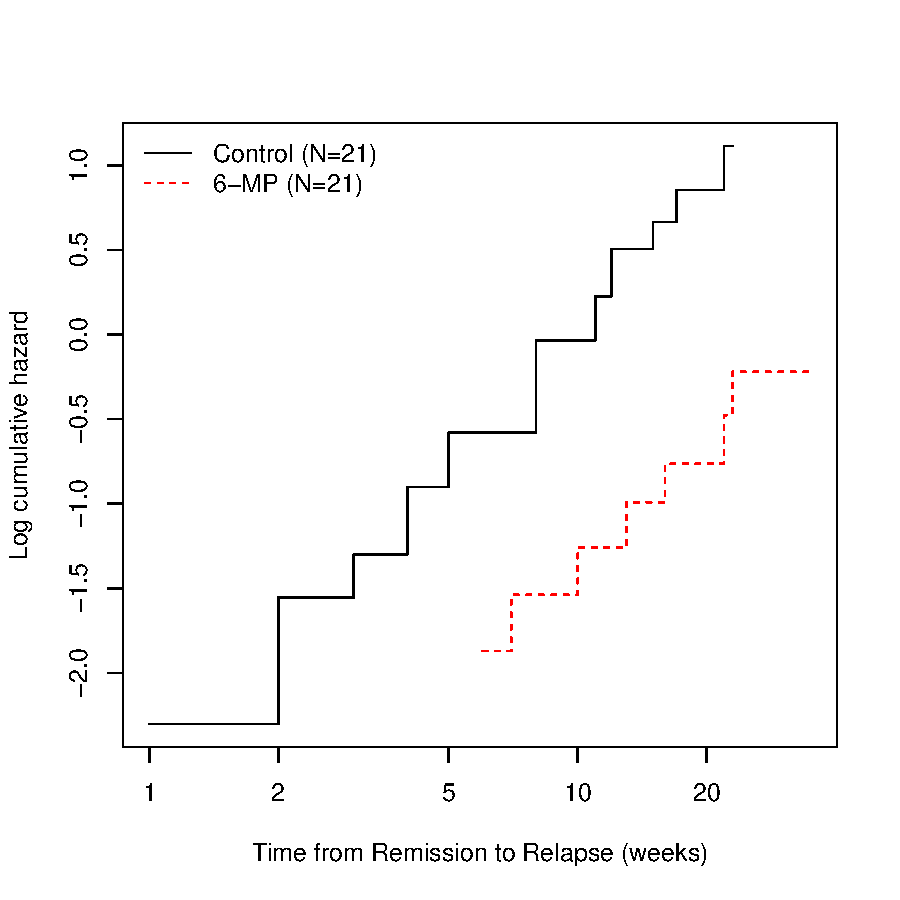
\includegraphics[scale=0.9]{leukemlogHaz.pdf}
		%\rule{35em}{0.5pt}
	\caption{Log cumulative hazard plot of treatment groups.}
	\label{figure1}
\end{figure}
Since the curves seem to be parallel, the proportionality assumption is very likely to hold.
\newpage 
\item Our goal is to fit the following model
\begin{align}
\lambda(t|\text{trt}) = \lambda_{0}(t)\exp\left\{\beta_{1}\text{trt}
+\beta_{2}(\text{trt}\times t)\right\}.\nonumber
\end{align}
Thus, using simple algebra we get that the hazard ratio is
\begin{align}
\dfrac{\lambda(t|\text{trt}=1)}{\lambda(t|\text{trt}=0)}
=\dfrac{\lambda_{0}(t)\exp\left\{\beta_{1}+\beta_{2}t\right\}}{\lambda_{0}(t)\exp\left\{\beta_{1}\cdot0+\beta_{2}t\cdot0\right\}}
=\exp\left\{\beta_{1}+\beta_{2}t\right\}.
\nonumber
\end{align}
So, $\beta_{2}$ shows if the HR increases over time ($\beta_{2}>0$), or decreases over time ($\beta_{2}<0$). Once you have got estimates $\hat{\boldsymbol{\beta}}=(\hat{\beta}_{1},\hat{\beta}_{2})$, you can plot $\exp\left\{\hat{\beta}_{1}+\hat{\beta}_{2}t\right\}$ against time and see the shape of the hazard ratio over time.
An obvious but \textbf{incorrect} approach would be
\begin{spacing}{1.2}
\begin{footnotesize}
\begin{verbatim}
> # (b)-(ii): Incorrect model !!!
> fit = coxph( Surv(weeks,remiss) ~ trt + I(weeks*(trt=="6-MP")),data = leukem)
> summary(fit)
Call:
coxph(formula = Surv(weeks, remiss) ~ trt + I(weeks * (trt == 
    "6-MP")), data = leukem)

  n= 42, number of events= 30 

                               coef exp(coef) se(coef)      z Pr(>|z|)    
trt6-MP                     1.47927   4.38976  0.81291  1.820 0.068800 .  
I(weeks * (trt == "6-MP")) -0.18138   0.83412  0.05479 -3.311 0.000931 ***
---
Signif. codes:  0 ‘***’ 0.001 ‘**’ 0.01 ‘*’ 0.05 ‘.’ 0.1 ‘ ’ 1

                           exp(coef) exp(-coef) lower .95 upper .95
trt6-MP                       4.3898     0.2278    0.8923   21.5968
I(weeks * (trt == "6-MP"))    0.8341     1.1989    0.7492    0.9287

Concordance= 0.773  (se = 0.06 )
Rsquare= 0.534   (max possible= 0.988 )
Likelihood ratio test= 32.11  on 2 df,   p=1.066e-07
Wald test            = 15.19  on 2 df,   p=0.0005029
Score (logrank) test = 25.11  on 2 df,   p=3.532e-06
\end{verbatim}
\end{footnotesize}
\end{spacing}
A p-value of 0.0009 (measuring the interaction of treatment effect with time) is implausible given the shape of figure \eqref{figure1}, which clearly shows parallel curves. The issue is that the above code does not actually create a
time dependent covariate, rather it creates a time-static value for each subject based on their
value for the covariate \verb|weeks|.

After examining \verb|?coxph|, we can understand that we need to use the time transform functionality of \verb|coxph|, i.e., the \verb|tt| option. The \textbf{correct} code is
\begin{spacing}{1.2}
\begin{footnotesize}
\begin{verbatim}
> # You have to use the tt argumnent, 
> # Decode trt as a numeric variable
> leukem$trt = 1*(leukem$trt == "6-MP")
> fit = coxph( Surv(weeks,remiss) ~ trt + tt(trt),data = leukem, 
+              tt = function(x,t,...){x*t})
> summary(fit)
Call:
coxph(formula = Surv(weeks, remiss) ~ trt + tt(trt), data = leukem, 
    tt = function(x, t, ...) {
        x * t
    })

  n= 42, number of events= 30 

              coef  exp(coef)   se(coef)      z Pr(>|z|)  
trt     -1.5813338  0.2057005  0.7758258 -2.038   0.0415 *
tt(trt)  0.0008651  1.0008655  0.0616960  0.014   0.9888  
---
Signif. codes:  0 ‘***’ 0.001 ‘**’ 0.01 ‘*’ 0.05 ‘.’ 0.1 ‘ ’ 1

        exp(coef) exp(-coef) lower .95 upper .95
trt        0.2057     4.8614   0.04496    0.9411
tt(trt)    1.0009     0.9991   0.88687    1.1295

Concordance= 0.69  (se = 0.188 )
Rsquare= 0.322   (max possible= 0.988 )
Likelihood ratio test= 16.35  on 2 df,   p=0.0002813
Wald test            = 14.51  on 2 df,   p=0.0007053
Score (logrank) test = 17.69  on 2 df,   p=0.0001443
\end{verbatim}
\end{footnotesize}
\end{spacing}
Thus, the correct analysis shows that the hazard ratio does not vary over time as the coefficient of \verb|tt(trt)| is very close to zero and insignificant. However, keep in mind that this test has the power to detect a linear relationship of log(HR) with time. 
 
\end{enumerate}
\end{enumerate}

 